% Multi-round memory accumulation on two agent harnesses (results as of 2026-09-22).
% Figures are the current working (Chinese-labelled) exports; they will be redrawn
% in English before submission.  Source CSVs and plotting scripts are in the
% GitHub paper branch under results/multiround_20260922/.

\subsection{Multi-round memory accumulation on two agent harnesses}
\label{sec:multiround-two-harness}

To test whether distilled cross-round memory is useful outside one agent
implementation, we repeat the round-by-round protocol on two harnesses.
\textbf{MLEvolve} is the multi-agent search harness used in the rest of this
paper (planner, coder, reviewer, and an inner AgentTuner, with the frozen v7
runtime).  \textbf{autoresearch} is a port of a single-agent research loop:
one agent edits a candidate training script, the host executes it and keeps or
discards it; there is no MLEvolve searcher, reviewer, or inner agent.  The two
harnesses share only the memory-pack format (search-experience and
inner-tuning cards) and the execution container.

\paragraph{Protocol.}
Round~1 (R1) runs with no memory.  Each later round may read only memory cards
distilled from the earlier rounds listed in Table~\ref{tab:multiround-summary};
it never reads their code, checkpoints, or task packages.  Every round has a
7{,}200\,s budget and a 3{,}600\,s per-node cap, a single seed, and one fixed
internal split.  ``Host'' scores are recomputed by the host from a validated
checkpoint on a held-back \emph{search} split whose labels the agent never sees;
``tune'' scores are candidate-reported values on the agent-visible tune split.
None of these are Kaggle leaderboard scores, and the search split is used
adaptively across candidates within a run.

\begin{table*}[t]
  \centering
  \caption{Best score per round for the multi-round memory experiments
  (single seed per round; ``$\downarrow$'' lower is better, ``$\uparrow$''
  higher is better).  Memory column lists the rounds whose distilled cards
  were readable.  MLE = MLEvolve; AR = autoresearch.  All values are internal
  Host or tune scores, not Kaggle scores.}
  \label{tab:multiround-summary}
  \small
  \setlength{\tabcolsep}{4pt}
  \begin{tabular}{@{}lllll@{}}
    \toprule
    Harness & Task (metric) & Round & Memory read & Best score \\
    \midrule
    \multirow{5}{*}{MLE} & \multirow{5}{*}{Leaf (Host search log-loss $\downarrow$)}
      & R1 & none & 0.443894 \\
    & & R2 & R1 & 0.442665 \\
    & & R3 & R1+R2 & 0.066774 \\
    & & R5$^\dagger$ & R1--R4 (91 cards) & 0.042636 \\
    & & R6$^\dagger$ & R5 pack (repeat) & 0.035167 \\
    \midrule
    \multirow{4}{*}{MLE} & \multirow{4}{*}{Spooky (Host search log-loss $\downarrow$)}
      & A$^\dagger$ & none & 0.35620 \\
    & & C & A & 0.31031 \\
    & & D & A+B+C & 0.27670 \\
    & & E & A+B+C+D & 0.25928 \\
    \midrule
    \multirow{4}{*}{MLE} & \multirow{4}{*}{iMet 2020 (Host micro-F1 $\uparrow$)}
      & R1 & none & 0.42416 \\
    & & R2 & R1 & 0.50491 \\
    & & R3 & R1+R2 & 0.51130 \\
    & & R4 & R1+R2+R3 & 0.58865 \\
    \midrule
    \multirow{4}{*}{MLE} & \multirow{4}{*}{Plant Pathology 2021 (Host micro-F1 $\uparrow$)}
      & R1 & none & 0.83857 \\
    & & R2 & R1 & 0.85573 \\
    & & R3 & R1+R2 & 0.86316 \\
    & & R4 (repeat) & R1+R2+R3 & 0.86077 \\
    \midrule
    \multirow{3}{*}{AR} & \multirow{3}{*}{iMet 2020 (tune micro-F1 $\uparrow$)}
      & R1 & none & 0.38823 \\
    & & R2 & R1 & 0.43860 \\
    & & R3 & R1+R2 & 0.45849 \\
    \midrule
    \multirow{4}{*}{AR$^\ddagger$} & \multirow{4}{*}{Spooky (Host search log-loss $\downarrow$)}
      & R1 (MLE) & none & 0.35028 \\
    & & R2 & R1 & 0.35111 \\
    & & R3 & R1+R2 & 0.34911 \\
    & & R2 rerun & new AR R1 & 0.35625 \\
    \midrule
    \multirow{3}{*}{AR$^\ddagger$} & \multirow{3}{*}{Leaf (Host search log-loss $\downarrow$)}
      & R1 (MLE) & none & 0.44389 \\
    & & R2 & R1 & 0.06357 \\
    & & R3 (MLE) & R1 + orig.\ MLE R2 & 0.06677 \\
    \bottomrule
  \end{tabular}

  \vspace{2pt}
  {\footnotesize $^\dagger$Part of the budget was resumed after a provider
  outage with a different model, provider, or GPU host.
  $^\ddagger$Mixed series: only the rounds without the ``(MLE)'' tag ran on
  autoresearch; the MLE rounds are the memory sources or reference points.}
\end{table*}

\paragraph{MLEvolve: memory rounds reach better scores on all four tasks.}
On every MLEvolve task, the best memory-enabled round is better than the
no-memory R1 (Table~\ref{tab:multiround-summary}).  On Leaf
(Figure~\ref{fig:mle-leaf-rounds}), R1 and the one-round-memory R2 stay near
0.44 Host log-loss, whereas R3 reaches 0.0668 and the rounds reading the
91-card cumulative pack reach 0.0426 and 0.0352; the first certified R6
candidate already appears at about 13 minutes.  On Spooky
(Figure~\ref{fig:mle-spooky-acde}), Host log-loss decreases with each added
memory source, from 0.3562 (A) to 0.3103 (C), 0.2767 (D), and 0.2593 (E); D's inner-tuning trajectory starts below A's
final tune loss, and E ends with the lowest tune loss (0.2643).  On
iMet (Figure~\ref{fig:mle-imet-rounds}) Host micro-F1 increases from 0.4242 to
0.5049, 0.5113, and 0.5887.  On Plant Pathology
(Figure~\ref{fig:mle-pp21-rounds}) it increases from 0.8386 to 0.8557 and
0.8632; the R4 repeat (0.8608) is slightly below R3, so the gain saturates
after two memory rounds and is not monotone.

\paragraph{autoresearch: the same memory transfers to a single-agent loop.}
The cleanest cross-harness evidence is iMet on autoresearch
(Figure~\ref{fig:ar-imet-rounds}), where model, data split, runtime, and budget
are fixed across rounds.  The calibrated tune micro-F1 rises from 0.3882 (R1)
to 0.4386 (R2) and 0.4585 (R3), and the round best arrives earlier
(89.3, 79.6, and 65.3 minutes).  Host recomputation agrees
(0.3892, 0.4410, 0.4586).  On Leaf (Figure~\ref{fig:ar-leaf-rounds}), an
autoresearch R2 that reads memory distilled from the MLEvolve R1 reaches
0.0636 Host log-loss, compared with 0.4439 for that R1; one of its candidates
reproduces the R1 best exactly (0.443894), indicating that the recipe was
carried over by memory before being improved.  On Spooky
(Figure~\ref{fig:ar-spooky-rounds}) the effect is small: autoresearch R2 and R3
obtain 0.3511 and 0.3491 against 0.3503 for the MLEvolve R1 memory source,
and a rerun of R2 that read a new autoresearch R1 obtains 0.3562 after a
provider failure stopped it at about 60 minutes.

\paragraph{What these results do and do not show.}
These are descriptive single-seed trajectories, not controlled ablations.
Several confounds change together with memory:
(i) the model changes from Luna to Terra in the MLEvolve iMet and Spooky
chains and between harnesses on Leaf;
(ii) some rounds were resumed after provider outages on a different host or
provider (Leaf R5/R6, Spooky A/C, iMet R4), and several runs ended by a
watchdog rather than normally;
(iii) runtime patches were introduced between rounds (for example the iMet
recipe contract from R3 and the Plant Pathology R1 wall-clock versus later
effective-time budgets);
(iv) some series are curated: Leaf R4 and the original Leaf R2, Spooky B, the
first Plant Pathology R4, and lower-scoring iMet R2 attempts are omitted from
the figures, and the mixed autoresearch series pair autoresearch rounds with
MLEvolve reference rounds;
(v) an autoresearch no-memory Leaf rerun reached 0.0168 at a mid-run snapshot,
so the Leaf gap between R1 and later rounds cannot be attributed to memory
alone.
The consistent direction across four MLEvolve tasks and the clean
autoresearch iMet chain motivates a matched study with repeated seeds, fixed
model and runtime, and no-memory controls run under the same harness, which we
list as the next experiment.

\FloatBarrier
\begin{figure*}[t]
  \centering
  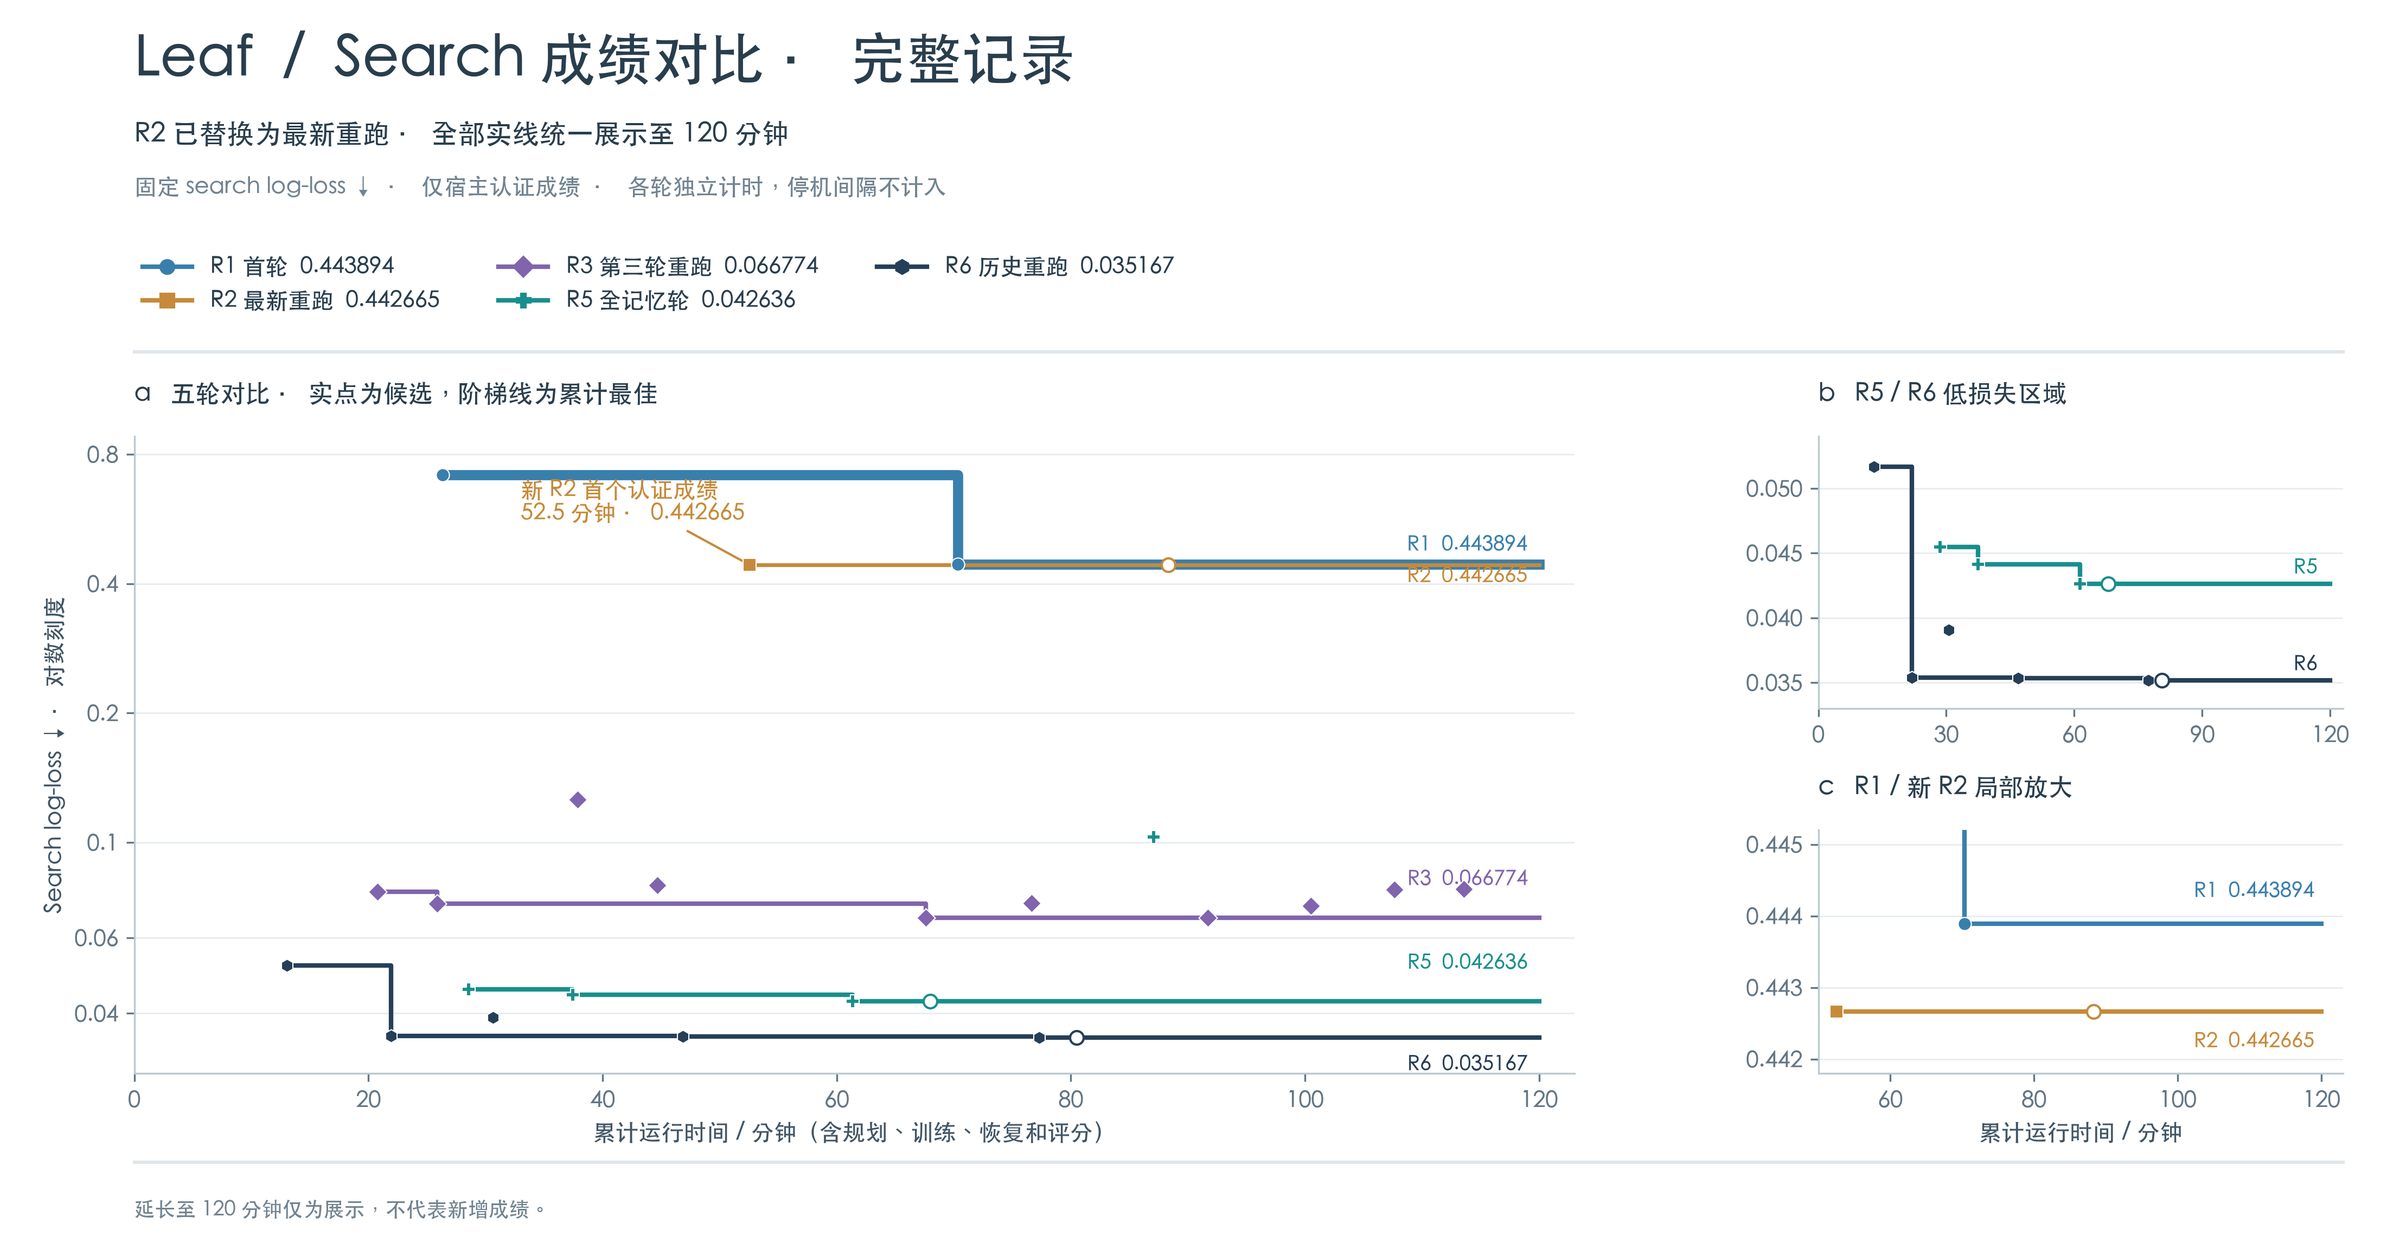
\includegraphics[width=\textwidth]{figures/multiround/mle_leaf_search_rounds.png}
  \caption{MLEvolve, Leaf: Host search log-loss (log scale, lower is better)
  against cumulative runtime for R1 (no memory), R2 (R1 memory, latest rerun),
  R3 (R1+R2), and R5/R6 (91-card cumulative pack; R6 repeats R5's condition).
  Points are certified candidates; step lines are running bests.  Lines are
  extended to 120 minutes for display only.  Panels b and c magnify the
  low-loss region and the R1/R2 overlap.}
  \label{fig:mle-leaf-rounds}
\end{figure*}

\begin{figure*}[t]
  \centering
  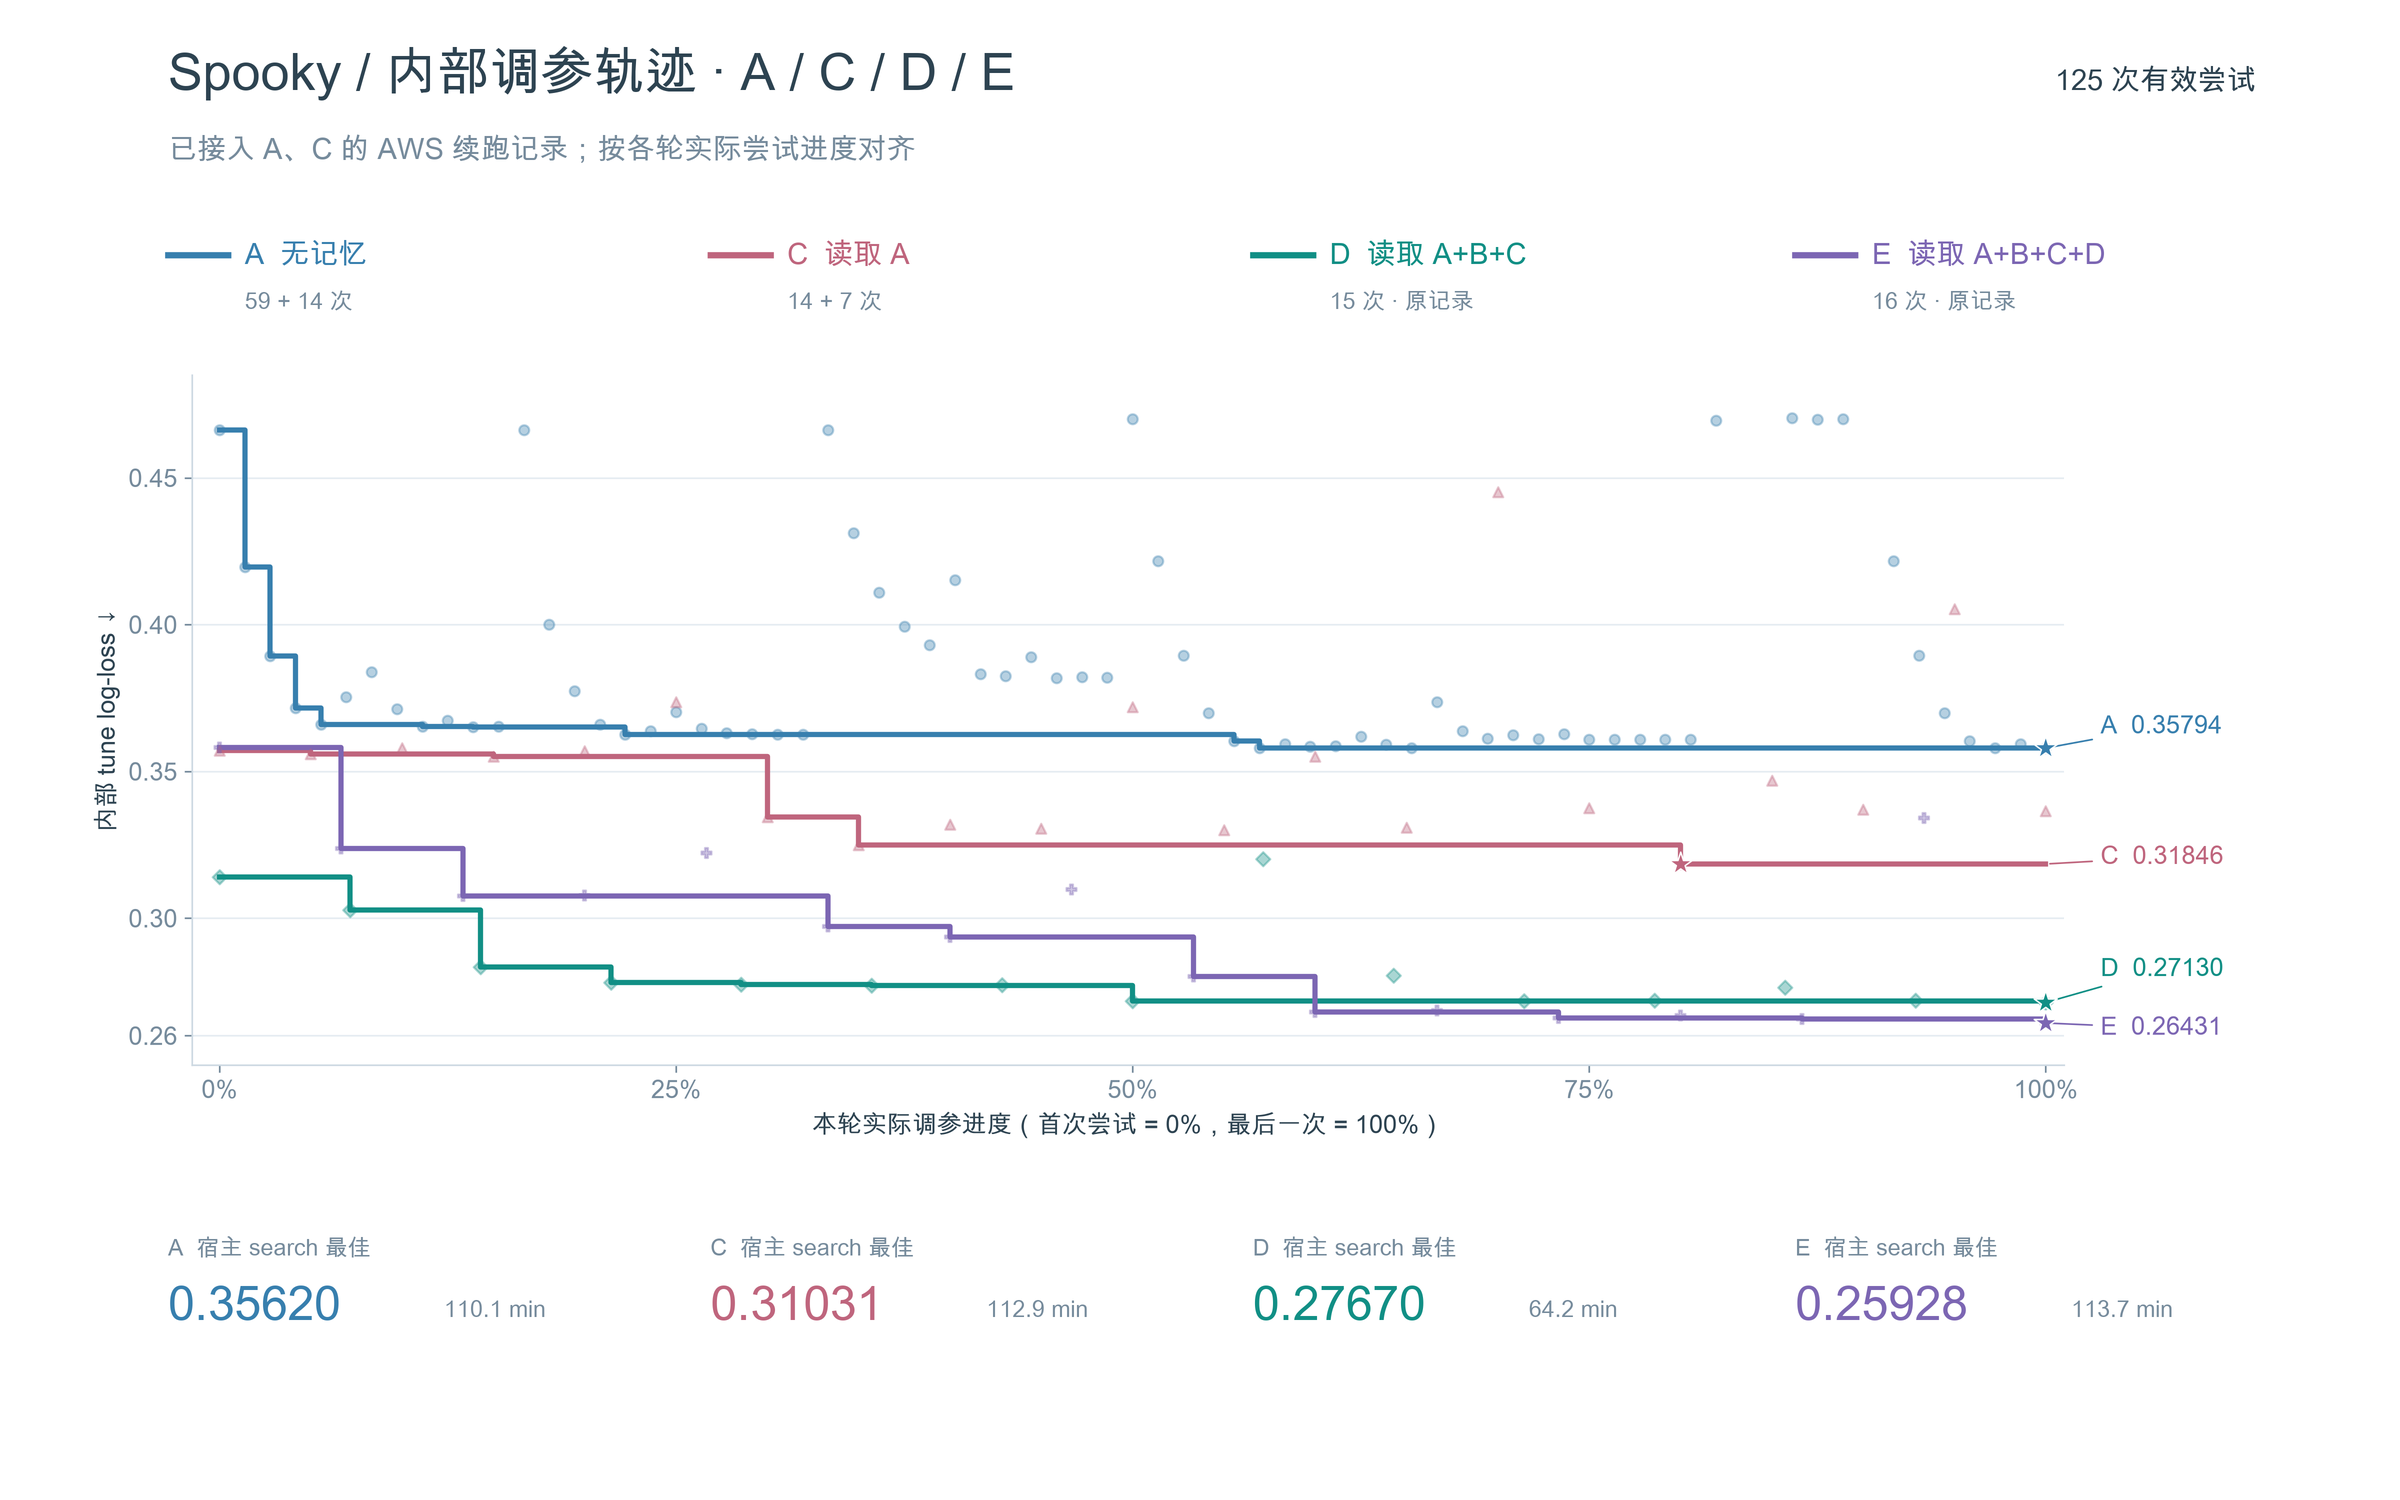
\includegraphics[width=\textwidth]{figures/multiround/mle_spooky_acde_inner.png}
  \caption{MLEvolve, Spooky Author Identification: inner-tuning log-loss
  (lower is better) against normalized attempt progress for A (no memory),
  C (reads A), D (reads A+B+C), and E (reads A+B+C+D); 125 valid trials.
  The footer reports each round's best Host search log-loss and its time.
  Round B is used as a memory source but not plotted.}
  \label{fig:mle-spooky-acde}
\end{figure*}

\begin{figure*}[t]
  \centering
  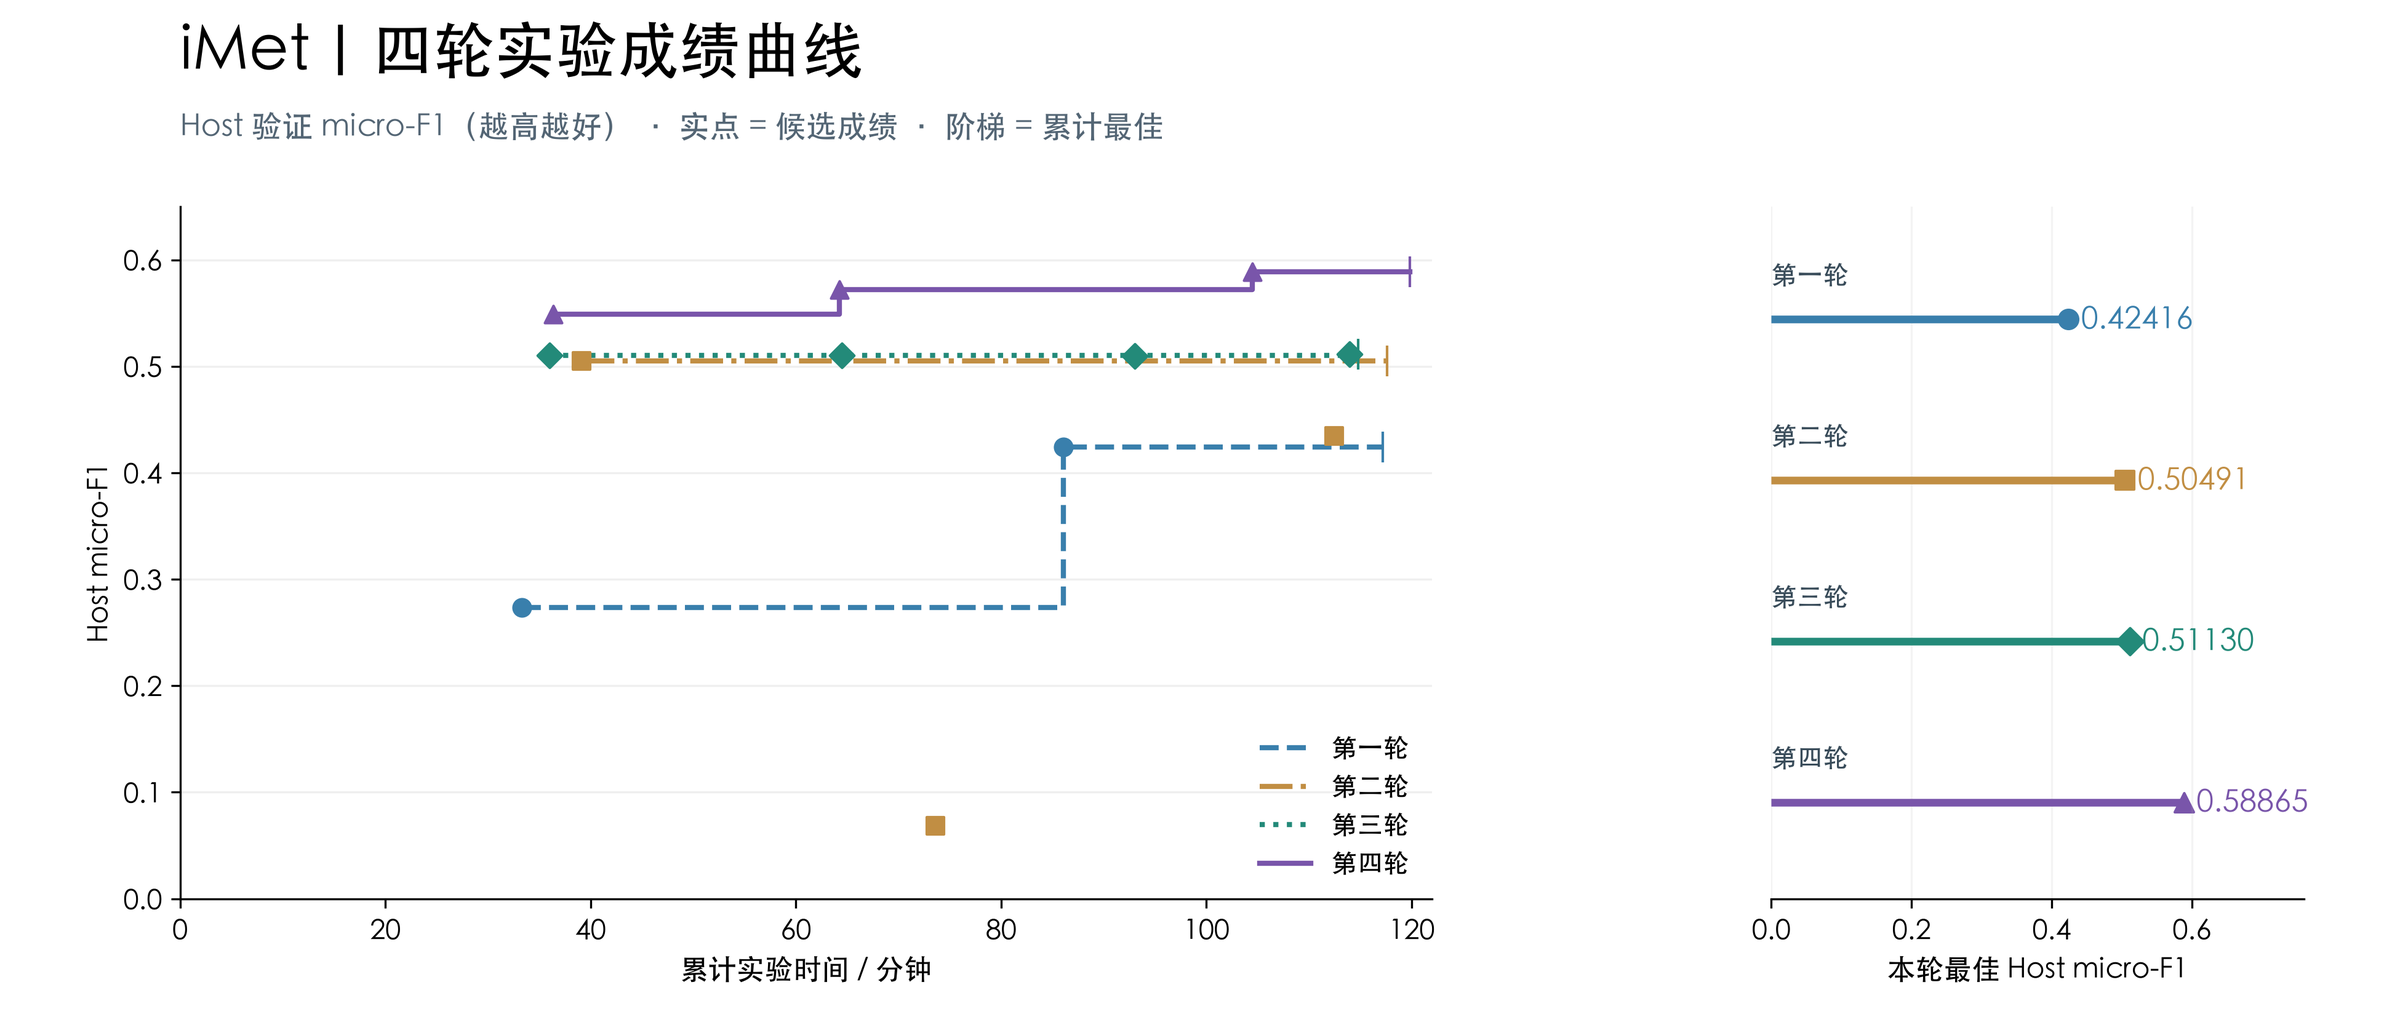
\includegraphics[width=\textwidth]{figures/multiround/mle_imet_four_rounds.png}
  \caption{MLEvolve, iMet 2020 FGVC7 (3{,}474 attributes): Host micro-F1
  (higher is better) against cumulative runtime for four rounds with
  increasing memory (none; R1; R1+R2; R1+R2+R3).  Points are
  checkpoint-validated, Host-recomputed candidates; step lines are running
  bests; the right panel shows each round's best.}
  \label{fig:mle-imet-rounds}
\end{figure*}

\begin{figure*}[t]
  \centering
  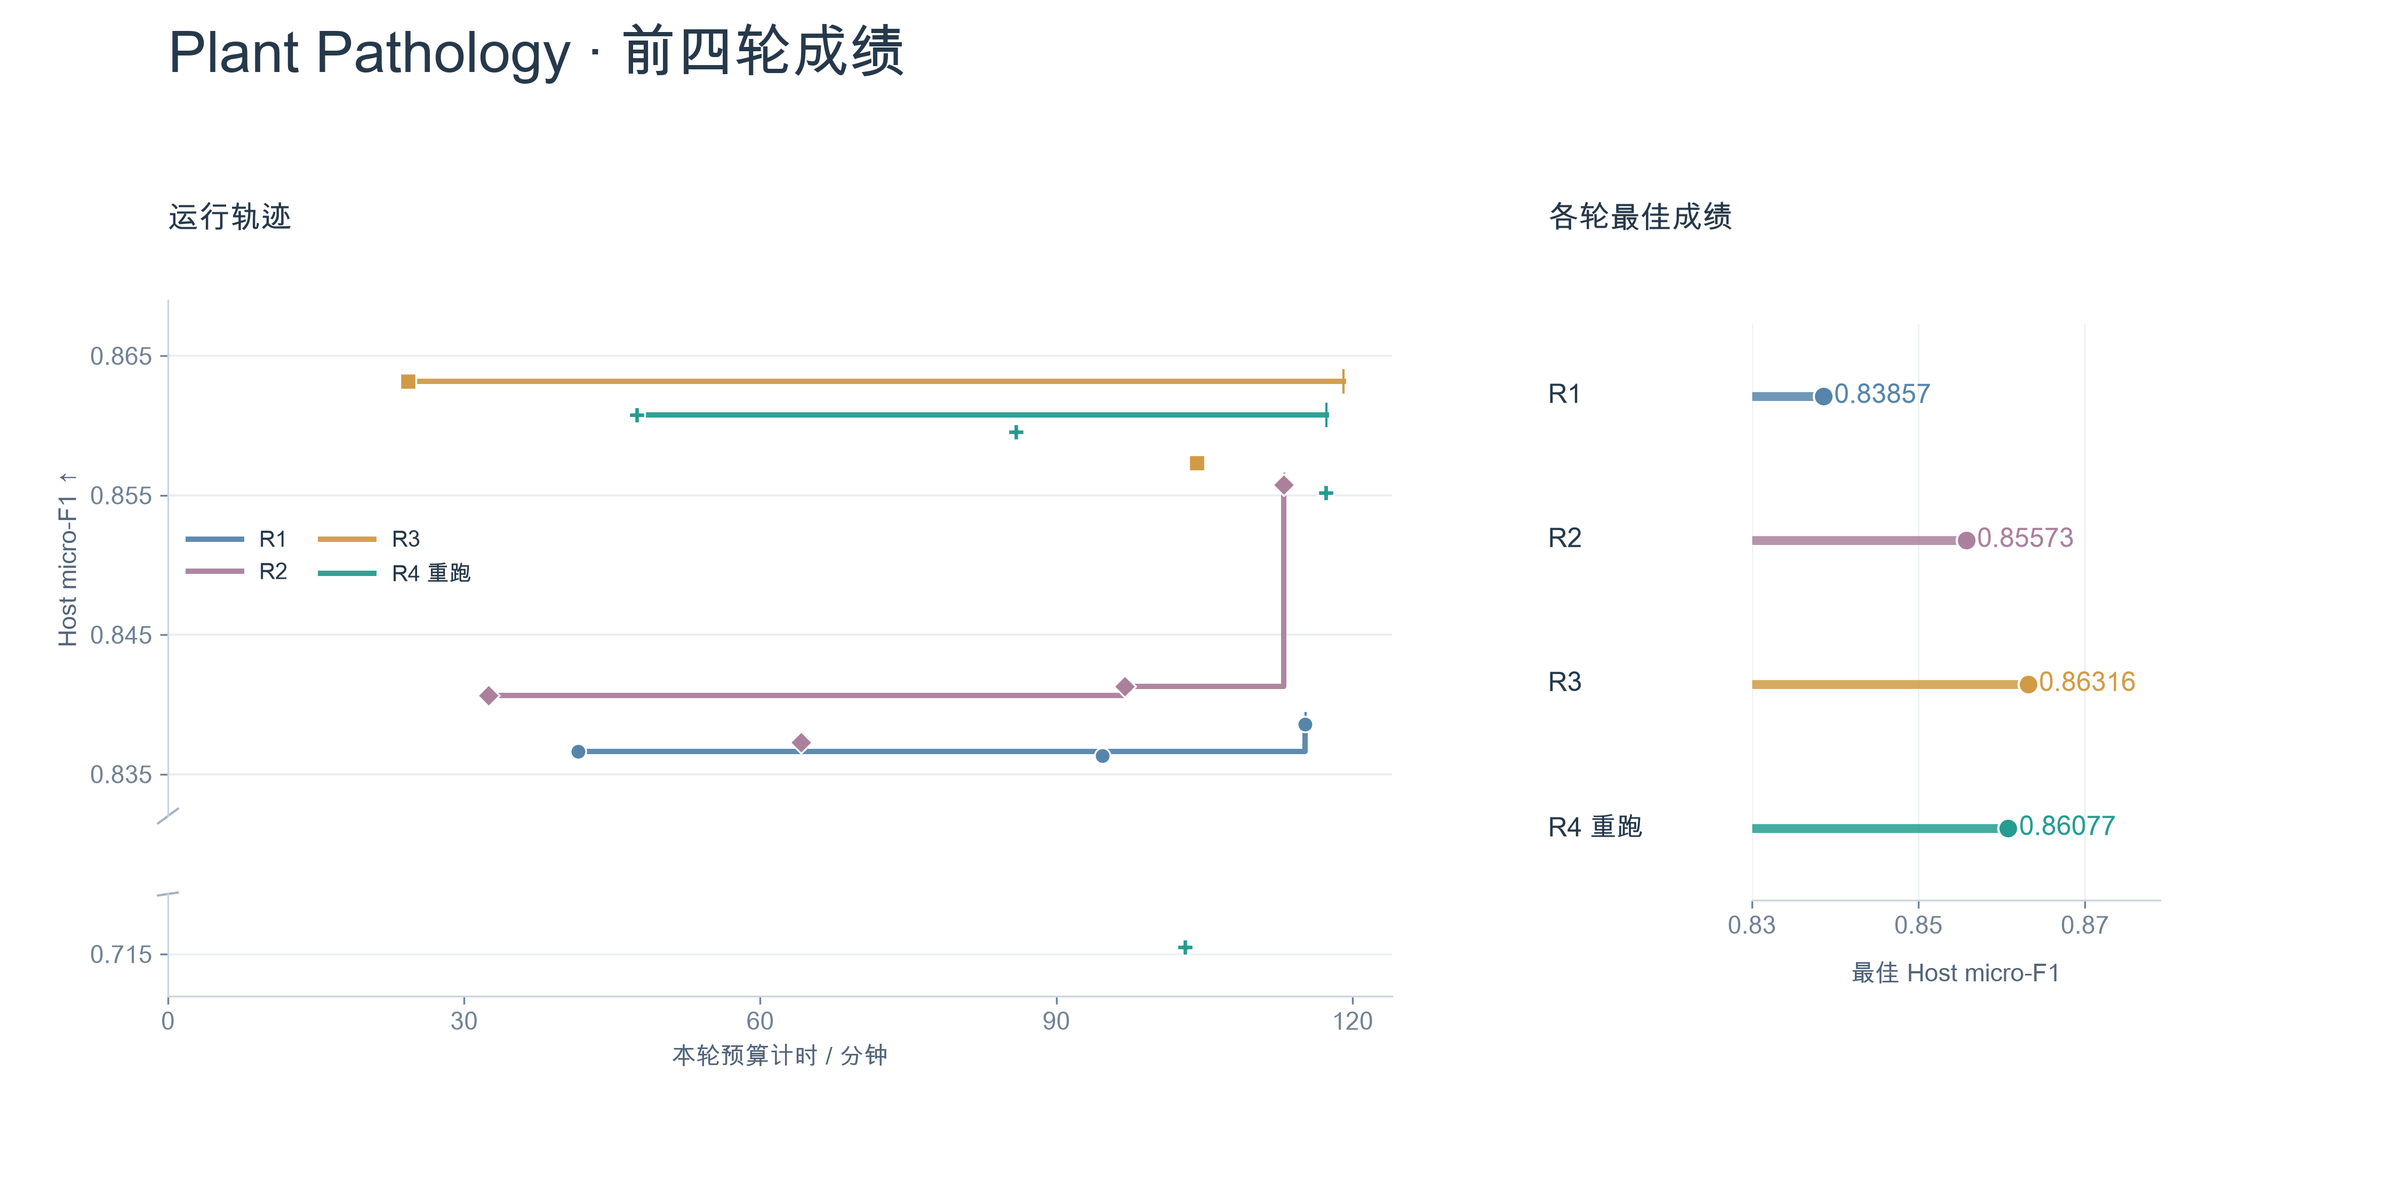
\includegraphics[width=\textwidth]{figures/multiround/mle_pp21_four_rounds.png}
  \caption{MLEvolve, Plant Pathology 2021 FGVC8 (six labels): Host micro-F1
  (higher is better) against budgeted runtime for R1 (no memory), R2 (R1),
  R3 (R1+R2), and the R4 repeat (R1+R2+R3).  The broken axis keeps one
  low-scoring R4 candidate (0.716) visible.}
  \label{fig:mle-pp21-rounds}
\end{figure*}

\begin{figure*}[t]
  \centering
  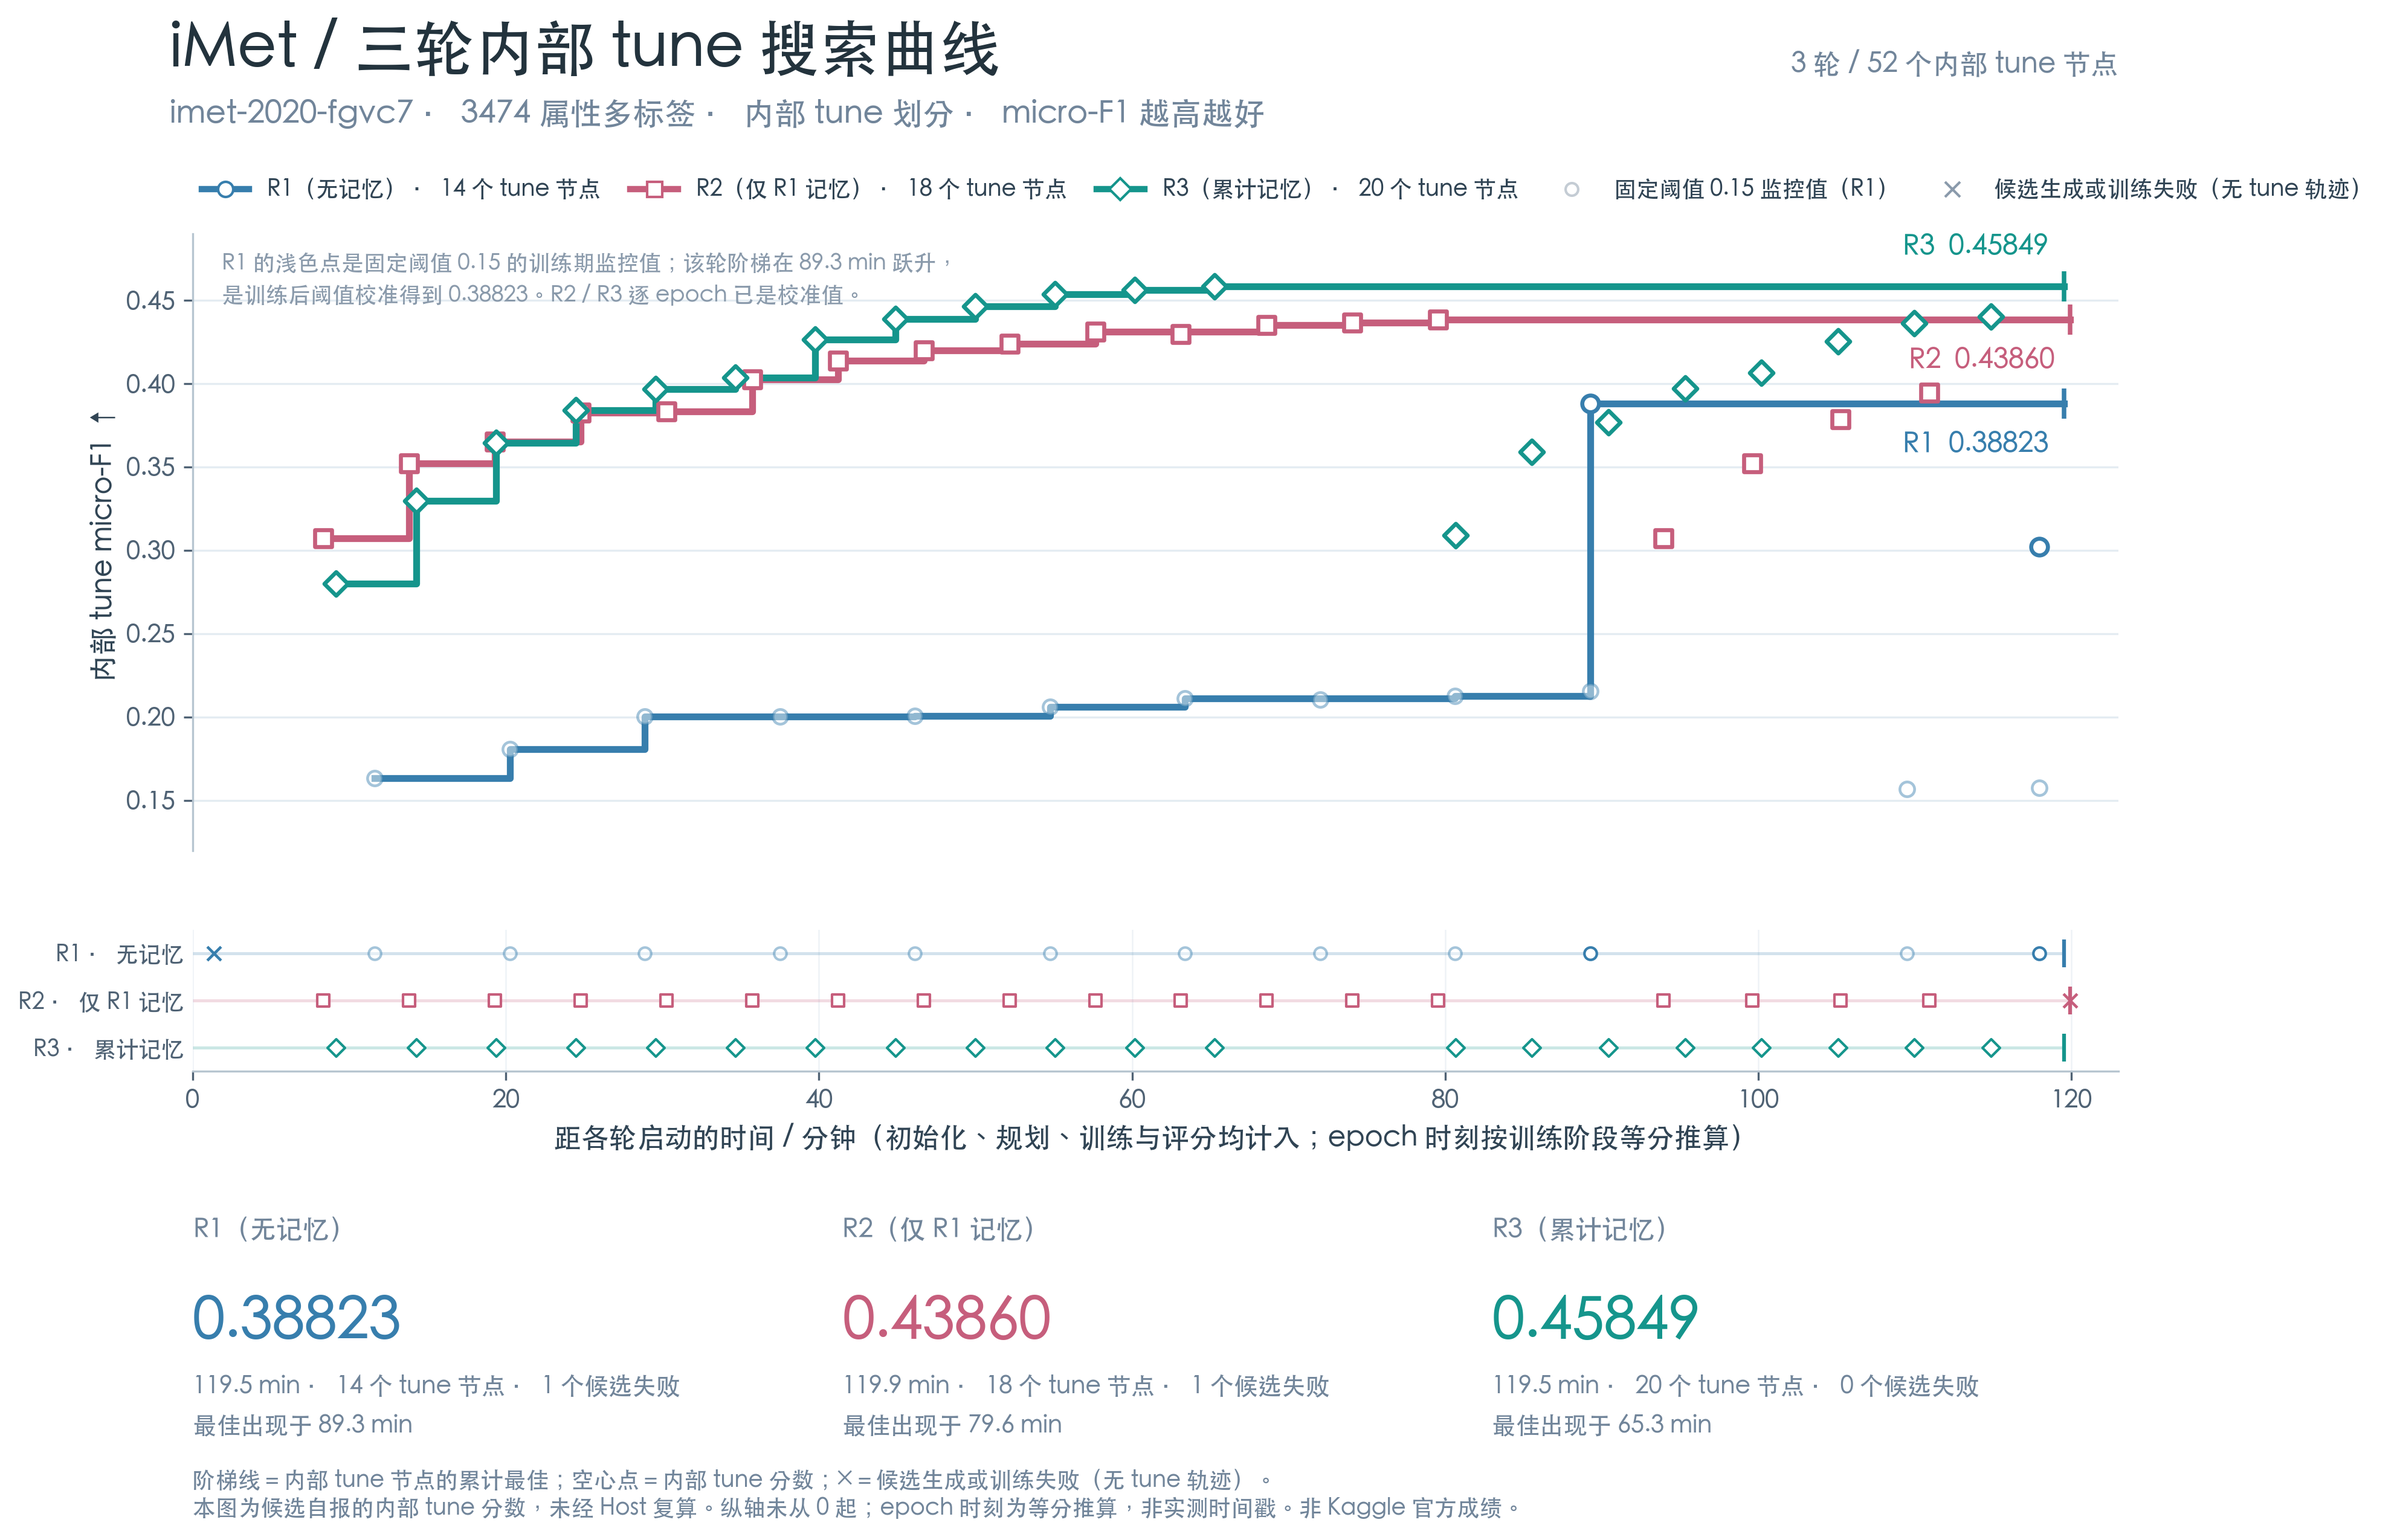
\includegraphics[width=\textwidth]{figures/multiround/ar_imet_three_rounds_tune.png}
  \caption{autoresearch, iMet 2020: internal tune micro-F1 (higher is better)
  for R1 (no memory), R2 (R1 memory only), and R3 (cumulative R1+R2), with
  52 tune nodes in total.  R1's light points are a fixed-threshold (0.15)
  training monitor and are not comparable with the calibrated values; epoch
  times are interpolated within each training stage.  The y-axis does not
  start at zero.}
  \label{fig:ar-imet-rounds}
\end{figure*}

\begin{figure*}[t]
  \centering
  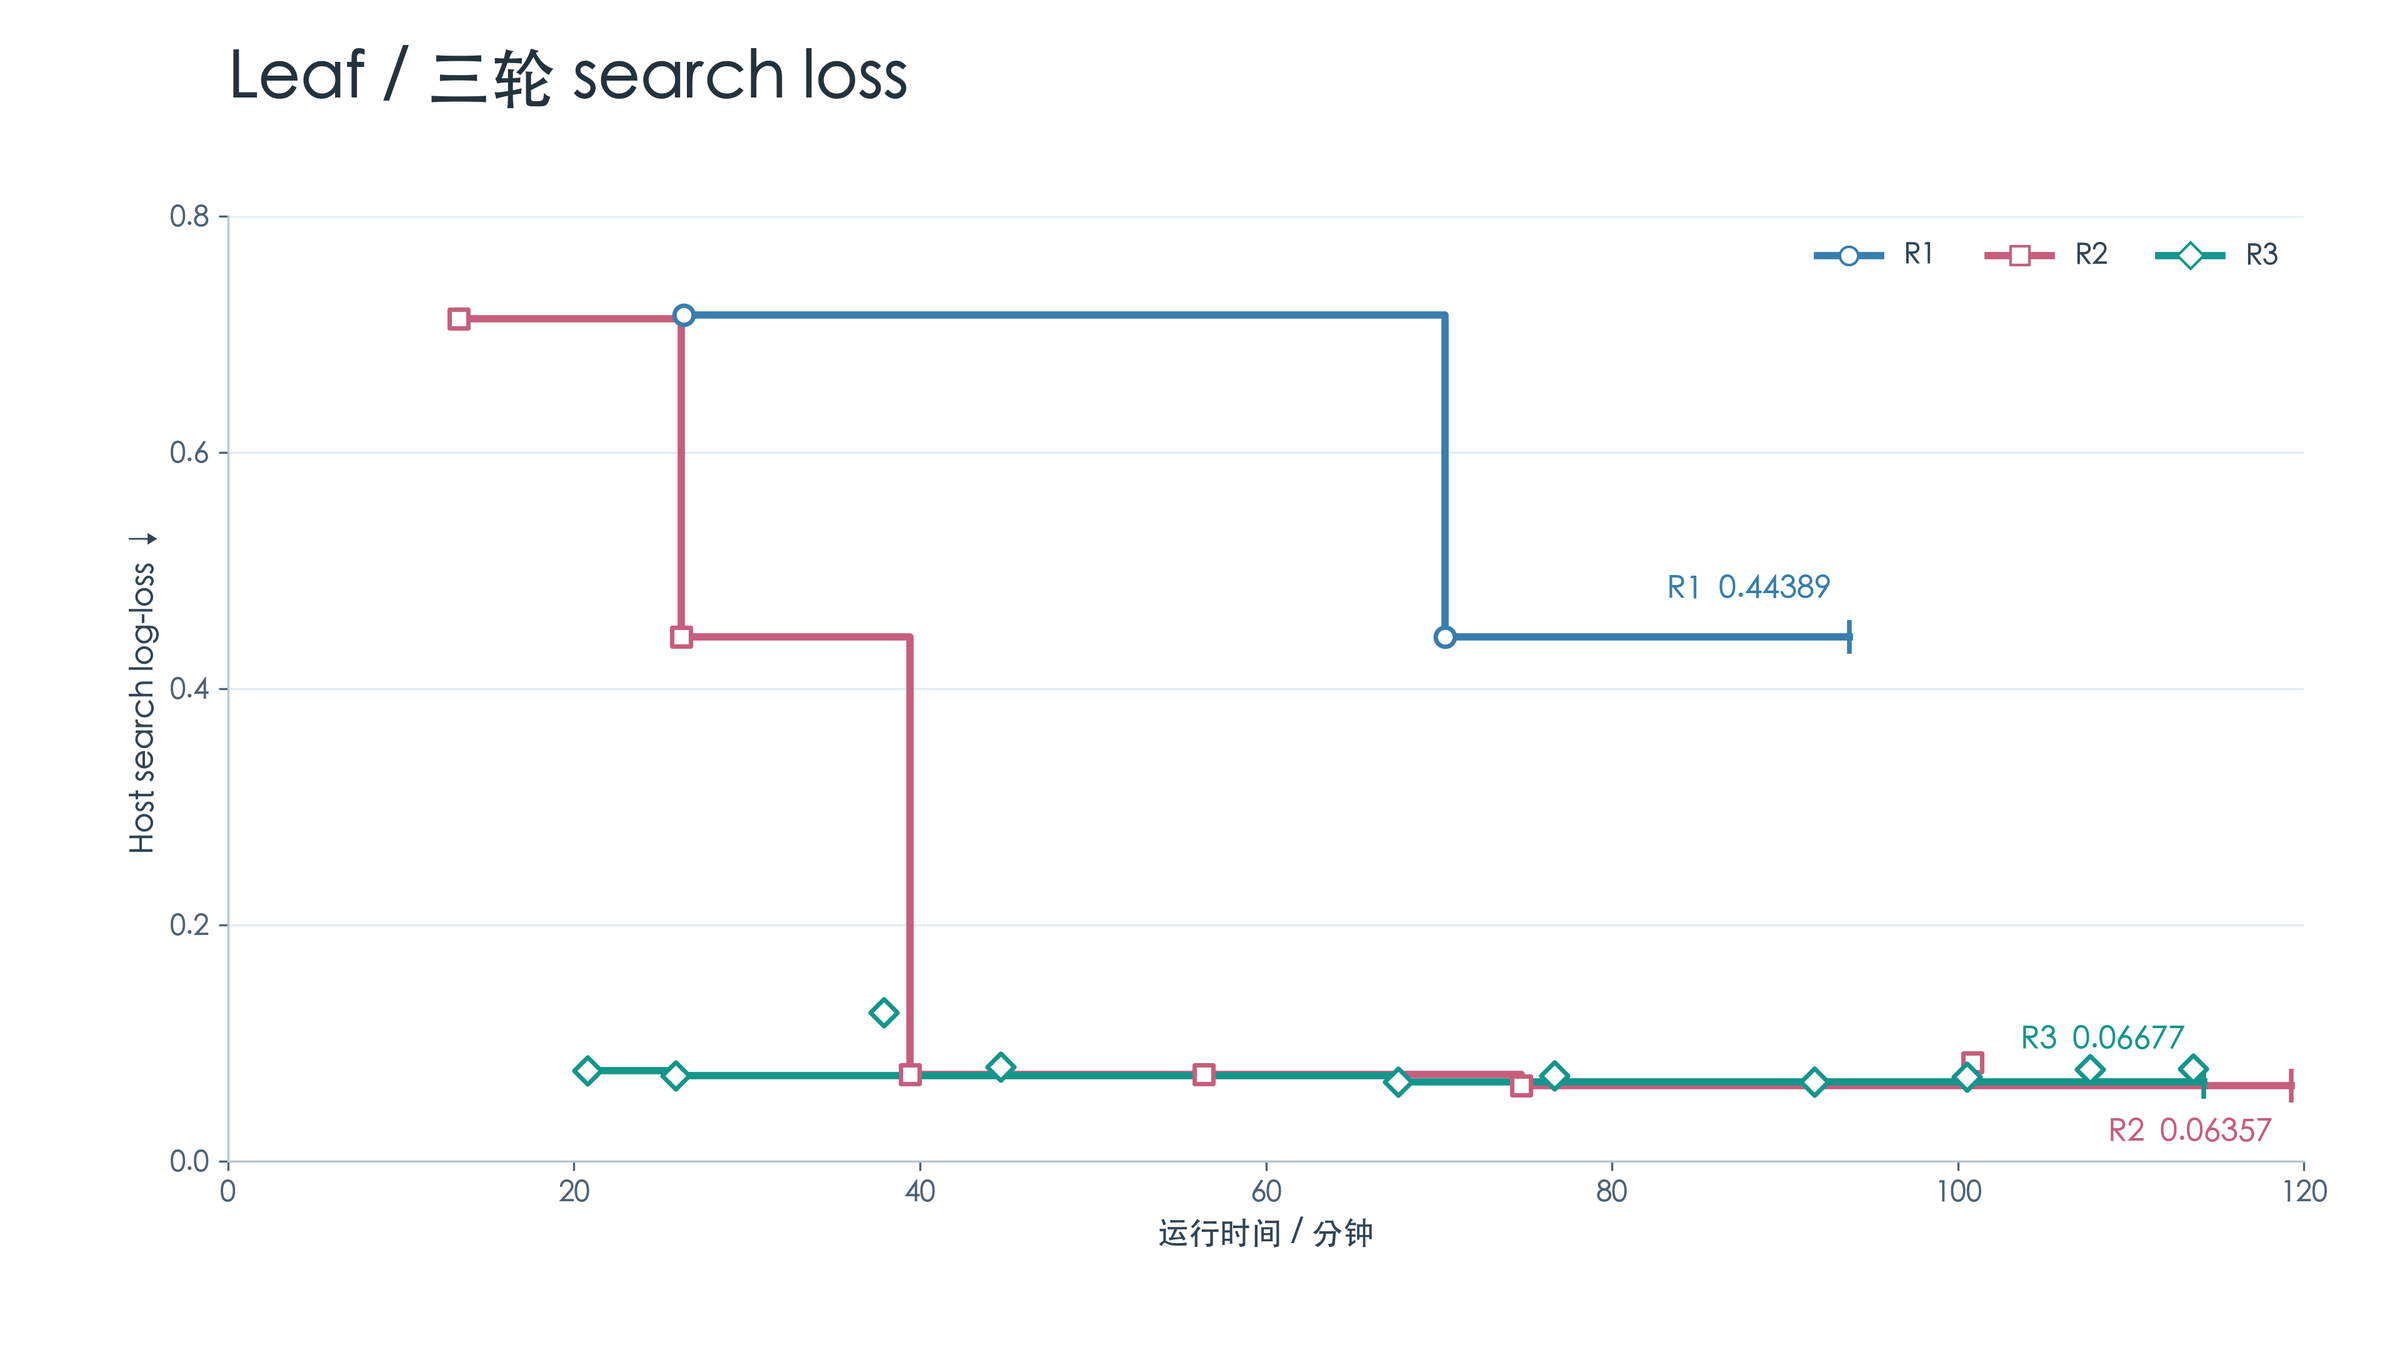
\includegraphics[width=0.85\textwidth]{figures/multiround/ar_leaf_three_rounds.png}
  \caption{Leaf, mixed series: Host search log-loss against runtime.  R2 is an
  autoresearch round that reads memory distilled from the MLEvolve R1; R1 and
  R3 are the MLEvolve rounds of Figure~\ref{fig:mle-leaf-rounds} (R3 reads the
  original MLEvolve R2, not the plotted autoresearch R2).}
  \label{fig:ar-leaf-rounds}
\end{figure*}

\begin{figure*}[t]
  \centering
  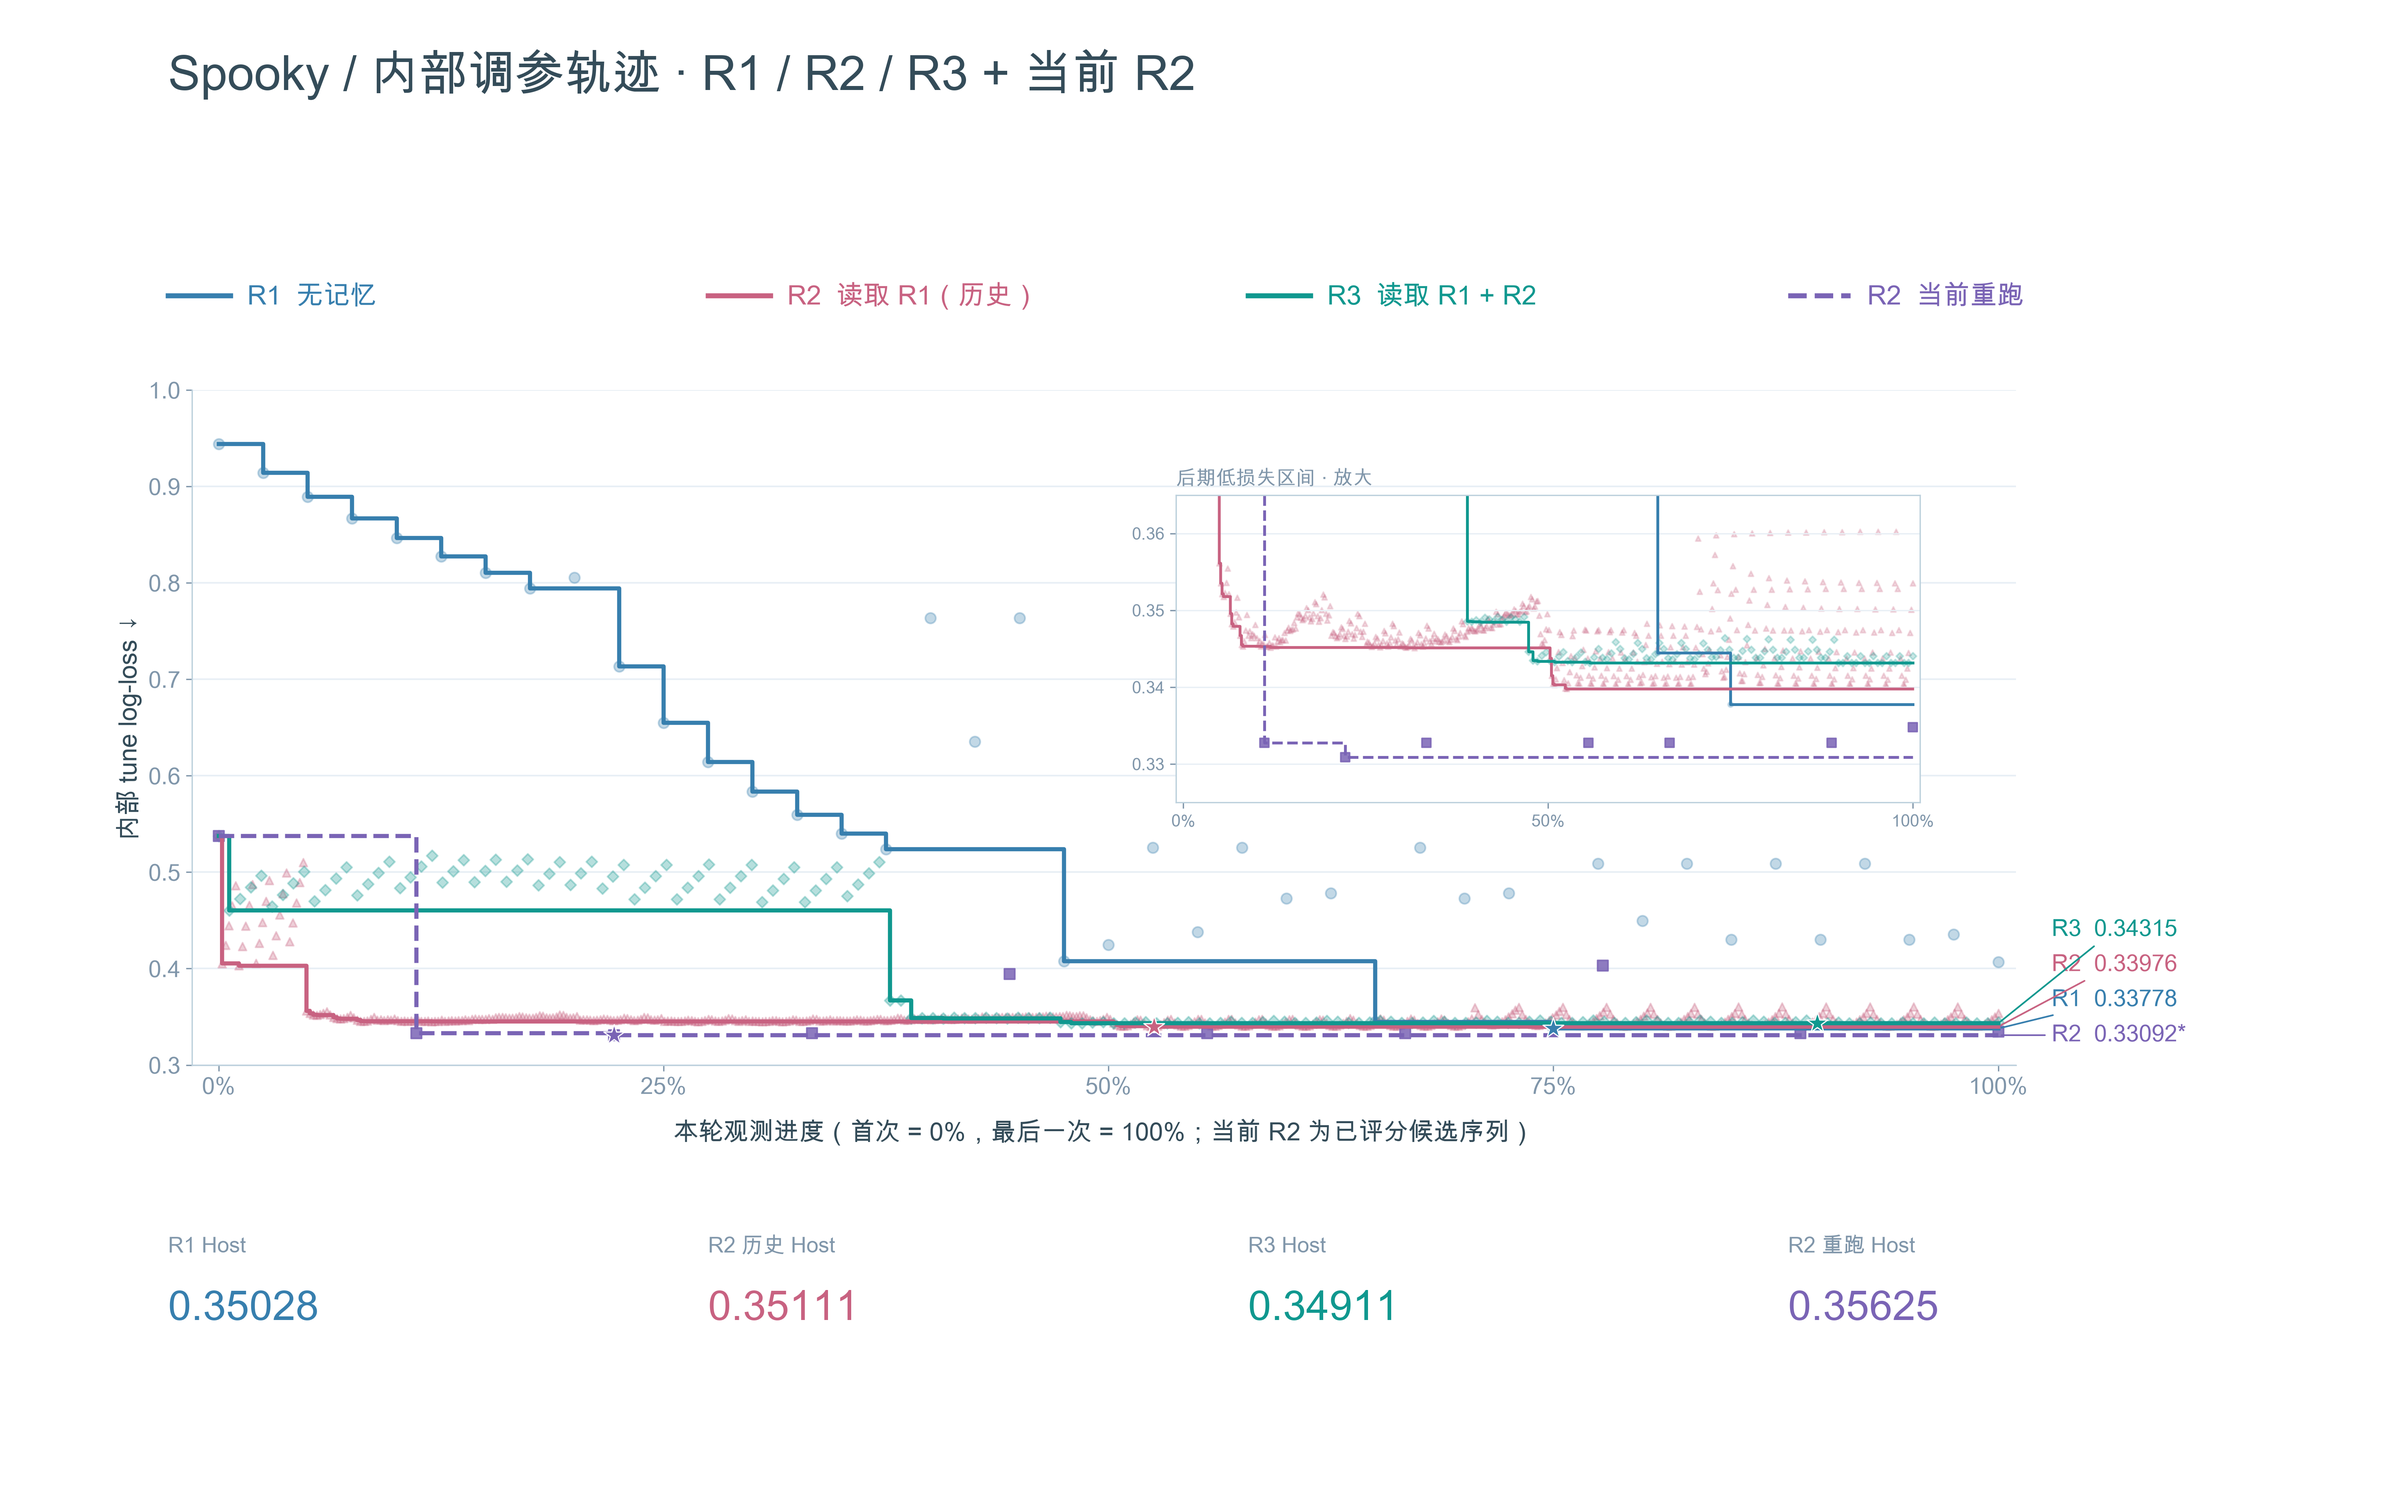
\includegraphics[width=\textwidth]{figures/multiround/ar_spooky_rounds.png}
  \caption{Spooky, mixed series: inner tune log-loss against normalized
  observation progress.  R1 is a historical MLEvolve run truncated to the
  7{,}200\,s budget; R2 (reads R1) and R3 (reads R1+R2) are autoresearch
  rounds; the dashed ``current R2'' is an autoresearch rerun that reads a new
  autoresearch no-memory R1 and stopped at about 60 minutes on a provider
  error.  The footer reports Host search log-loss.}
  \label{fig:ar-spooky-rounds}
\end{figure*}
\FloatBarrier
